\documentclass[../main.tex]{subfiles}
\begin{document}

\subsection{Datasets}
In this project two diferent datasets provided by the hospital clinic
have been used to train and validate the despeckle and stain models:
one for the \gls{cm} domain and one for the \gls{he} domain.

The Python implementation of all the datasets used can be found at appendix
\ref{appendix:datasets}

\paragraph{\gls{cm} set}
The \gls{cm} dataset consists of 27 large slides (around 100,000,000 pixels),
each corresponing to a different sample of skin tissue.
Some of this slides contain artifacts around the edges; in order to not
provide this noise to the models, the slides are manually cropped avoiding
this artifacts and focusing on the area containing the tissue.
Working with such a large images is not practical since they do not fit
in most GPUs' memory. A simple script to extract overlaping 1024x1024
patches out of the slides is developed so that, along with ``on-the-fly''
data augmentation techniques (random crop and random flip), more information
can be extracted from the dataset.
Only patches with a minimum mean grey level on both modes are extracted to
be sure that they contain tissue texture.
From that, a random sample of 1000 patches is used as a training set.

\paragraph{\gls{he} set}
The \gls{he} dataset contains a total of 560 crops of 1024x1024 pixels from
whole slide histopathological images.

\subsection{Despeckling network}
\label{sec:despeckling-network}
As explained in section \ref{sec:speckle-noise}, \gls{rcm} contain artifacts
caused by a multiplicative noise (see figure \ref{fig:speckle} for an example).
In this section different noise models are
described and then the proposed methods for mitigating it are presented.

\subsubsection{Speckle noise}
As a means of having pairs of noisy-clean images needed to train a denoising
model, \gls{fcm} are artificially contaminated with a noise model.
In SAR imaging, where speckle noise also appears, the noise is modeled by
a gamma distribution with unit mean and variance $\frac{1}{L}$ (assuming
the image is an average of $L$ \emph{looks})
(\cite{GammaSpeckle}):
\begin{equation}\label{eq:gamma-distribution}
F \sim \Gamma(k = L, \theta = \frac{1}{L})
\end{equation}

\begin{figure}[h]
\centering
\begin{subfigure}{.3\textwidth}
  \centering
  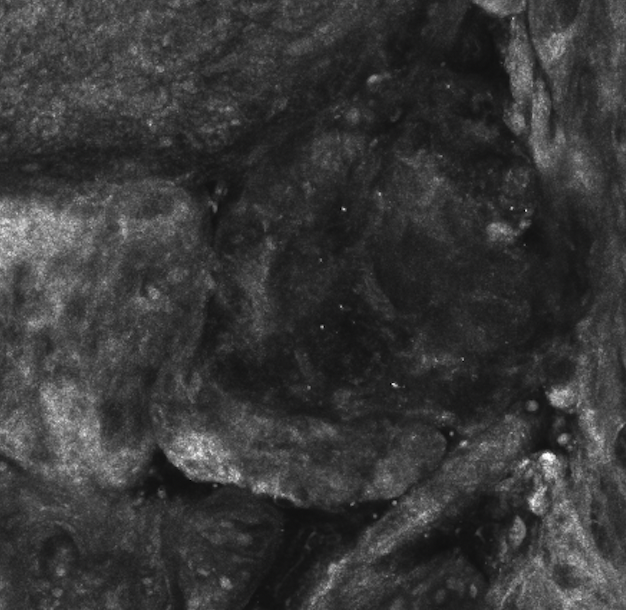
\includegraphics[width=.8\linewidth]{speckle-1}
\end{subfigure}%
\begin{subfigure}{.3\textwidth}
  \centering
  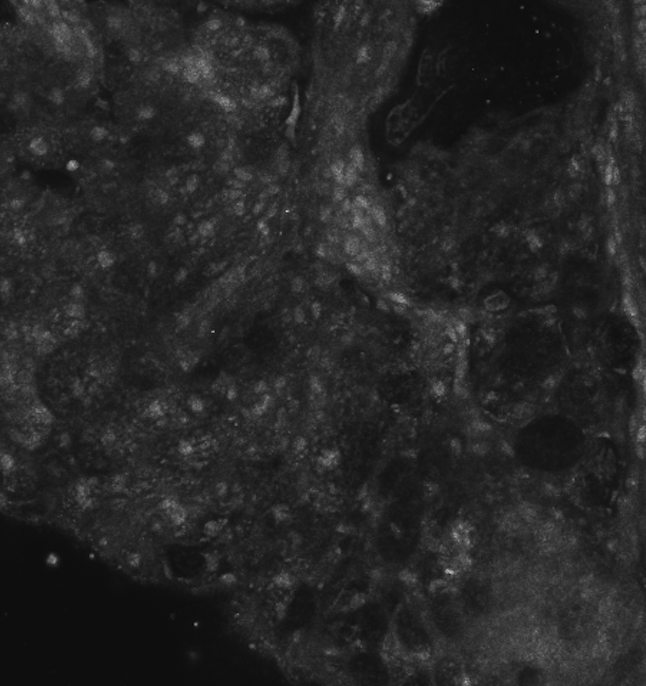
\includegraphics[width=.8\linewidth]{speckle-2}
\end{subfigure}%
\begin{subfigure}{.3\textwidth}
  \centering
  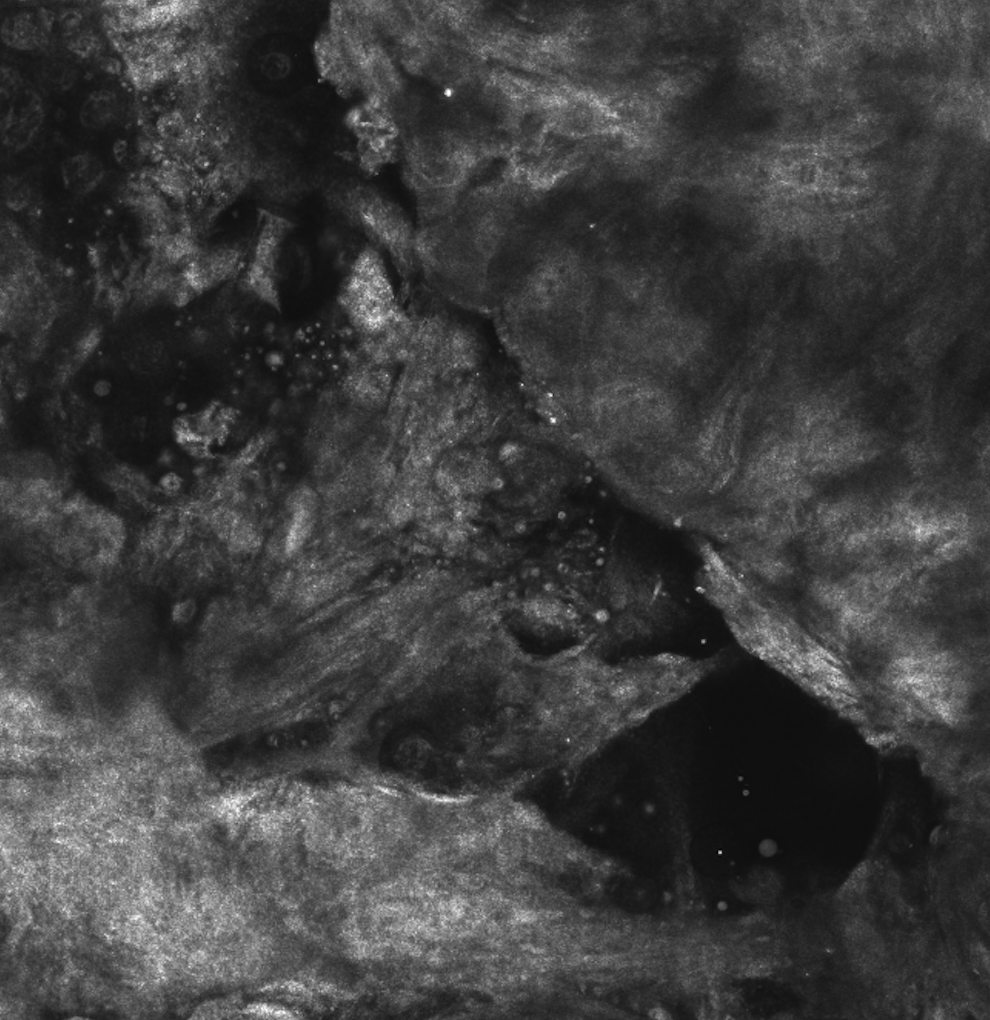
\includegraphics[width=.8\linewidth]{speckle-3}
\end{subfigure}
\caption{Three example of RCM images contaminated with speckle noise}
\label{fig:speckle}
\end{figure}

Other models for the noise distribution exist; for instance, MATLAB's
Image Processing Toolbox uses a uniform distribution with mean 1 and
variance 0.05:
\begin{equation}
F \sim U(0.6535,1.3464)
\end{equation}

In the case of ultrasound imaging a rayleigh distribution with mean 1 is used
(\cite{RayleighSpeckle}):
\begin{equation}
F \sim Rayleigh(\sigma=\sqrt{\frac{2}{\pi}})
\end{equation}

Based on the appearence of artificially contaminated \gls{fcm} images compared to
naturally contaminated \gls{rcm}, the experiments on this work are based on the
gamma model \eqref{eq:gamma-distribution}.

\subsubsection{Proposed network architectures}
In order to filter the speckle noise, several \glspl{dnn} with the same basic
structure are defined. Inspired by the ResNet (\cite{he2015deep}) they all share a
\emph{skip connection} between the first and last layer of a \gls{cnn} similar to
\cite{Wang2018} approach for SAR imaging despeckling.

The code for the PyTorch implemetations of all the models can be found at
appendix \ref{appendix:despeckling}

\begin{figure}[H]
\centering
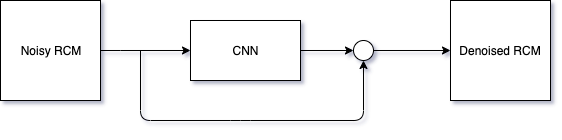
\includegraphics[width=0.9\linewidth]{despeckling-network}
\caption{Skeleton of the despeckling networks. The node at the output of the
CNN is the so-called residual connection, no operation is marked because
the different variations are precisely defined by it.}
\label{fig:despeckling-network}
\end{figure}

The \gls{cnn} block consists of $M$ convolutional layers each with $K$ filters
of size $N \times N$ and parametric \glspl{relu} activation functions
(\cite{he2015delving}),
except for the last layer which has one $1 \times 1$ filter to ``merge'' all
the channels of the previous layer into a single channel image.
Versions with and without an activation function are also defined.

The different model variations apply a distinct operation in the skip connection:
\begin{enumerate}
  \item Division skip connection: A element-wise division between
  the input image and the network's output is defined,
  so that it makes a prediction of the noise. A priori this model seems prone
  to suffer an unstable training.
  \item Multiplicative skip connection: A element-wise multiplication between
  the input image and the network's output is defined,
  so that it makes a prediction of the inverse of the noise.
  Although this estimation is more complicated, it is a ``safer'' alternative
  to the previous one.
  \item Additive skip connection: A ``classical'' skip connection where matrix
  summation between the input and output of the network is performed.
  In this case, the operation is done in the log-space ---the logarithm
  is applied to the input image and exponentiation to the model's output---
  in order to turn the noise into an additive one so is possible for the
  model to remove it.
\end{enumerate}

\subsection{Stain network}\label{sec:stain-network}

Obtaining aligned/paired data for \gls{cm} to \gls{he} is not possible since
tissue blocks scanned with the CM need to undergo slicing
before staining with H\&E; hence,
the staining models follow the \gls{cyclegans} framework introduced in section
\ref{sec:gans-translation}.

The discriminator model used is the PatchGAN (\cite{Zhu2017a}), the motivation
behind this model is to model high-frequency ``correctness''; this is done
by classifying (\emph{real/fake}) small patches of the image
(instead of the whole image) and averaging
all the responses to privide the definitive output of the distriminator.

For the generator model a baseline is defined along with two families of
advanced models.

\subsubsection{Baseline}\label{sec:stain-baseline}
The baseline generator is a learned version of the affine transformation
defined in \eqref{eq:affine-transformation}.
It is implemented as a single convolutional layer
with 3 filters of size 1 so each output pixel's channel is a linear combination
of the \gls{rcm} and \gls{fcm} values of the corresponding pixel of the
source \gls{cm} image plus a bias term.

\subsubsection{Advanced models}
Both families follow an encoder-decoder
structure, i.e.: a series of convolution layers with down-sampling (encoder)
followed by the same number of layers with up-sampling\footnotemark{} (decoder),
presumably the encoder maps the input into a latent representation where
semantic transformations can be more easily defined and then the decoder
``brings'' it back to the image space.

Instead of directly using the \gls{cm} modes, the digital staining
method proposed in \cite{Gareau2009} is used as source images for the geneators.
The reason is twofold: on the one hand to provide more similar sets so that
the mapping can be easier to learn, on the other hand, applying the
identity loss demands for domains with equal number of channels.

\begin{enumerate}
  \item ResNet-like generator: This model has the folling structure:
  \begin{itemize}
    \item First layer: The input image is first mirror padded to mantain its
    dimensions, it is then convolved with 64 $7 \times 7$ filters, the output
    is normalized with an instance normalization layer
    (\cite{ulyanov2016instance}) and followed by a \gls{relu} activation function.

    \item Down-sampling: This layer is composed by 3 2-strided
    (see down-sampling method \ref{n-strided-conv} in page
    \pageref{n-strided-conv}) convolution
    layers with exponentially increasing number of kernels of shape $3 \times 3$
    with instance normalization and \gls{relu} after each layer. So after this
    block, the signal will have 512 channels and the height and width will
    be reduced by a factor of 8 (e.g., if the input image has size
    $256 \times 256$, the output will be $32 \times 32$).

    \item Residual blocks: In a residual block, intead of trying to learn
    a transformation $\mathcal{T}(\tensor{x})$, the residual
    $\mathcal{F}(\tensor{x})$ is learnt so that
    $\mathcal{T}(\tensor{x}) = \mathcal{F}(\tensor{x}) + \tensor{x}$
    (ilustrated in figure \ref{fig:residual-block});
    the motivation behind this is to
    avoid the problem know as the degradation problem where deeper \gls{ann}
    perform worse than shallower counterparts.\\
    The generator network contains $R$ two-layer residual blocks between
    the encoder and the decoder also with \gls{relu} activation and
    instance normalization.

The last two blocks are the ``mirror image'' of the first two, i.e.:

    \item Up-sampling: 3 ``up-convolution'' layers with exponentialy decreasing
    number of filters so that the result is the same size as the original image.

    \item Final layer: Finally, the result of the previous layer is convolved
    by 3 $7 \times 7$ filters and a tanh activation function is used to
    bound the output's range.
  \end{itemize}

  \item UNet-like generator: The UNet (\cite{Ronneberger2015}) is a
  fully-convolutional network originally designed for medical image segmentation,
  it differs from standard encoder-decoder network in how the decoder
  reconstructs the image from the latent representation:
  \begin{itemize}
  \item Encoder: The encoder follows the same structure as the first two layers
  of the above described ResNet. No residual blocks are defined between the
  encoder and the decoder.
  \item Decoder: As a means to obtain low-level information
  (location, texture, ...) from the encoder,
  the output from the corresponding encoder layer is concatenated to the output
  of the previous decoder layer (figure \ref{fig:unet-diagram})
  \end{itemize}
\end{enumerate}

\begin{figure}[t]
\centering
\begin{minipage}{.5\textwidth}
\centering
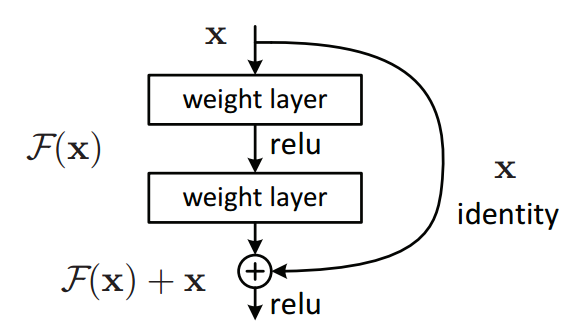
\includegraphics[width=0.8\linewidth]{residual_block}
\captionof{figure}{Residual block with 2 convolutional layers project.
Note that $\tensor{x}$ and $\mathcal{F}(\tensor{x})$ should be of the
same shape}
\label{fig:residual-block}
\end{minipage}%
\begin{minipage}{.5\textwidth}
\centering
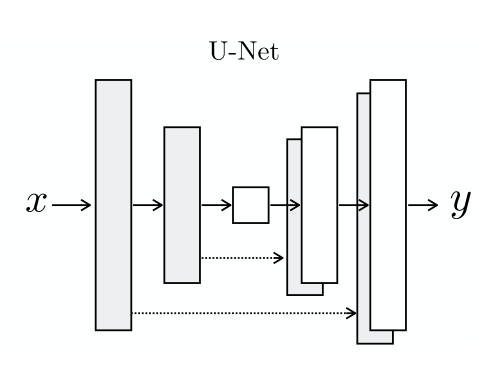
\includegraphics[width=0.7\linewidth]{unet-diagram}
\captionof{figure}{Skip connections between the UNet encoder and decorder}
\label{fig:unet-diagram}
\end{minipage}
\end{figure}

Both families use transposed convolutions\footnotemark[\value{footnote}]{}
in the decoder network.

\footnotetext{Different methods for up-sampling can be used: the more classical
interpolation methods (e.g., nearest neighbour or bicubic) or a
\emph{learnable} alternative called transposed convolution \cite{noh2015learning}
(also known as fractionally strided convolution and sometimes wrongly refered
to as deconvolution in some \gls{dl} publications.).
Chapter 4 of \cite{dumoulin2016guide} is suggested for readers not familiar
with this operation.}

\subsection{Inference technique}\label{sec:inference}
Whole slide images are too large to fit directly on a GPU, therefore,
the inference has to be tile-by-tile to obtain the stain transformed result.
This introduces artifacts (see figure \ref{fig:tiling-example}) between
adjacent tiles in the output due to
instance normalization relying on tile statistics.
In order to fix this issue, the WSI inference technique from \cite{Bel2019}
is applied.

\begin{figure}[b]
\centering
\begin{minipage}{.5\textwidth}
\centering
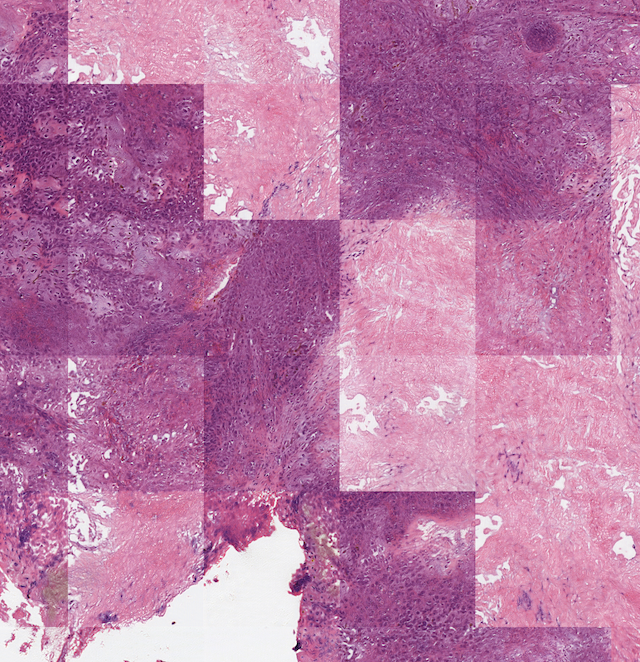
\includegraphics[width=0.5\linewidth]{tiling-example}
\captionof{figure}{Tiling artifacts when infering whole slides tile-by-tile}
\label{fig:tiling-example}
\end{minipage}%
\begin{minipage}{.5\textwidth}
\centering
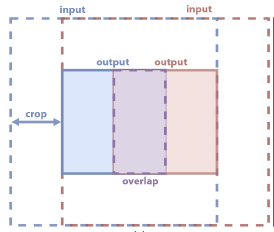
\includegraphics[width=0.5\linewidth]{inference}
\captionof{figure}{Inference is performed on a large input,
after which half of the image is cropped. The window is shifted by quarter of
the size, creating an overlap between tiles.}
\label{fig:inference}
\end{minipage}
\end{figure}

So as to have neighbouring tiles with similar statistics,
the method feeds overlapping regions to the model.
The steps are the following (ilustrated in figure \ref{fig:inference}):
\begin{enumerate}

\item A large $N \times N$ patch (e.g. $2048 \times 2048$) is transformed.

\item The borders are cropped to obtain the center of half the size of the input:
$\frac{N}{2} \times \frac{N}{2} = M \times M$.

\item The next prediction is made for a patch a quarter of the size apart from
      the previous one, i.e. the cropped output will have an overlap of 50\%
      with the previous one.

\item The crops are combined by multiplying (element-wise) by a weight matrix
      and adding them.  Two choices for this matrix are made:
\begin{enumerate*}[label=\itshape\alph*\upshape)]
\item An ``all 0.25'' matrix:
$\tensor{W} = 0.25 * \tensor{1}$
\item The outer-product of two translated triangular functions of length $M$:
$\left[ \tensor{W} \right]_{m,n} =
\Lambda(\frac{m}{M / 2} -1)\Lambda(\frac{n}{M / 2} -1)$
\label{n-strided-conv}
\end{enumerate*}

A version with non-overlapping outputs is also developed where only the inputs
overlap, instead of shifting the window by a quarter it is shifted by the half of
the input. In this case the number of iterations to infer the whole slide is
halved.
\end{enumerate}

\subsection{Quantitative measurement}
Evaluating generator models is not straightforward, as metrics for image
quality and diversity are dificult to define. Different methods are used
for comparing methods: The inception score (IS)
(\cite{DBLP:journals/corr/SalimansGZCRC16}) is used for measuring the quality
of generated samples, the Fréchet Inception Distance is supposed to improve on
the IS by comparing the statistics of generated samples to real samples.
In this work, a texture descriptor is used to try to measure if the generated
samples contain structures that are not present in the source image
(popularly known as hallucinations). An example of an hallucination of a 
model during a failed training is shown in figure \ref{fig:hallucination_B}.

The idea is to compare the input and output wholeslides by patches in a
texture sense. This is done by computing a texture descriptor of the luminance
of the source and the stained version and then computing a distance of the two.
After trying various posibilities, the chosen texture descriptor is the
\gls{lbp} histogram (\cite{lbp}).

\gls{lbp} is a gray-level invariant feature extractor that assigns a number
to every set of 9 neighboring pixels ---a central pixel and its 8
closest pixels--- in an image (in general, any number of pixels can be used but
9 is used here). The number is based on the difference of intensities between
the neighbors and the central pixel: a 1 is assigned on pixels with a grey-level
greater or equal than the center and 0 otherwise, this creates a code for each
pixel in the image ---by reading the assigned values clockwise starting at the
top left corner as a binary word--- that encodes the different posible edges.
An histogram of this codes can be computed
to obtain a description of the patterns that are found in a given image or patch.

The distance between the result and source patches is measured using
the chi-squared distance between the normalized \gls{lbp} histograms.

For reference purposes, the patch transformation depicted in figure
\ref{fig:hallucination} has a distance of 0.11.

\begin{figure}[h]
\centering
\begin{subfigure}{.5\textwidth}
  \centering
  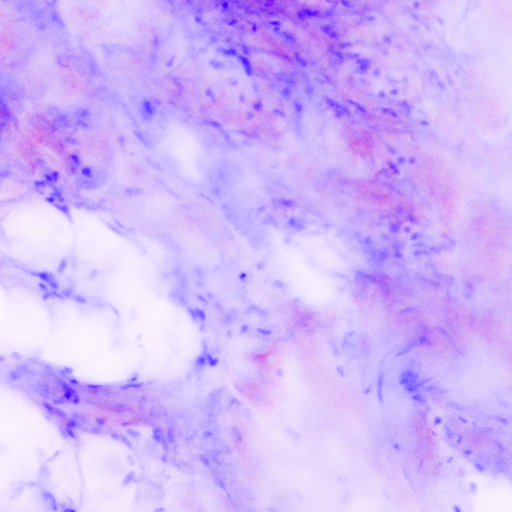
\includegraphics[width=.5\linewidth]{epoch246_real_A}
  \caption{Linearly stained sample}
  \label{fig:hallucination_A}
\end{subfigure}%
\begin{subfigure}{.5\textwidth}
  \centering
  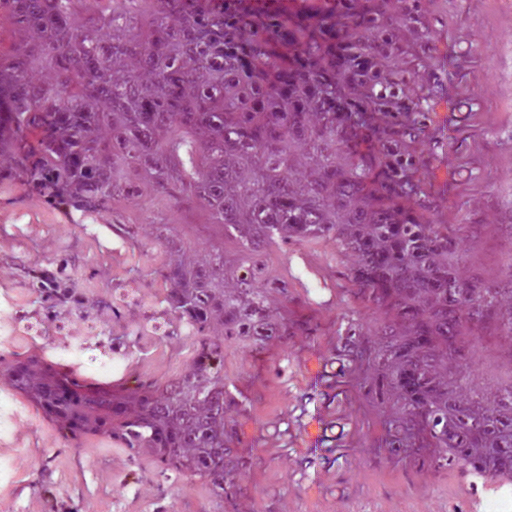
\includegraphics[width=.5\linewidth]{epoch246_fake_B}
  \caption{Transformed sample with hallucinations}
  \label{fig:hallucination_B}
\end{subfigure}
\caption{(a) is the input of the model that produces the output (b)}
\label{fig:hallucination}
\end{figure}



\end{document}
